% -*- mode: latex; mode: flyspell; ispell-local-dictionary: "en_US"; coding: utf-8; fill-column: 80 -*-

\documentclass{article}

\usepackage[utf8]{inputenc}
\usepackage[english]{babel}

\usepackage{amsmath,amsfonts,amssymb}
\usepackage{fullpage}
\usepackage{verbatim}

\usepackage{tikz,pgfplots}

\pgfplotsset{
  width=150mm,height=100mm,
  major grid style={thin,dotted,color=black!50},
  minor grid style={thin,dotted,color=black!50},
  grid,
  every axis/.append style={
    line width=0.5pt,
    tick style={
      line cap=round,
      thin,
      major tick length=4pt,
      minor tick length=2pt,
    },
  },
  legend cell align=left,
  legend pos=north west,
}

%%%%%%%%%%%%%%%%%%%%%%%%%%%%%%%%%%%%%%%%%%%%%%%%%%%%%%%%%%%%%%%%%%%%%%%%%%%%%%%%

\begin{document}

\title{Sorting Speed Example}
\author{Timo Bingmann}
\maketitle

% IMPORT-DATA stats stats.txt

\begin{center}
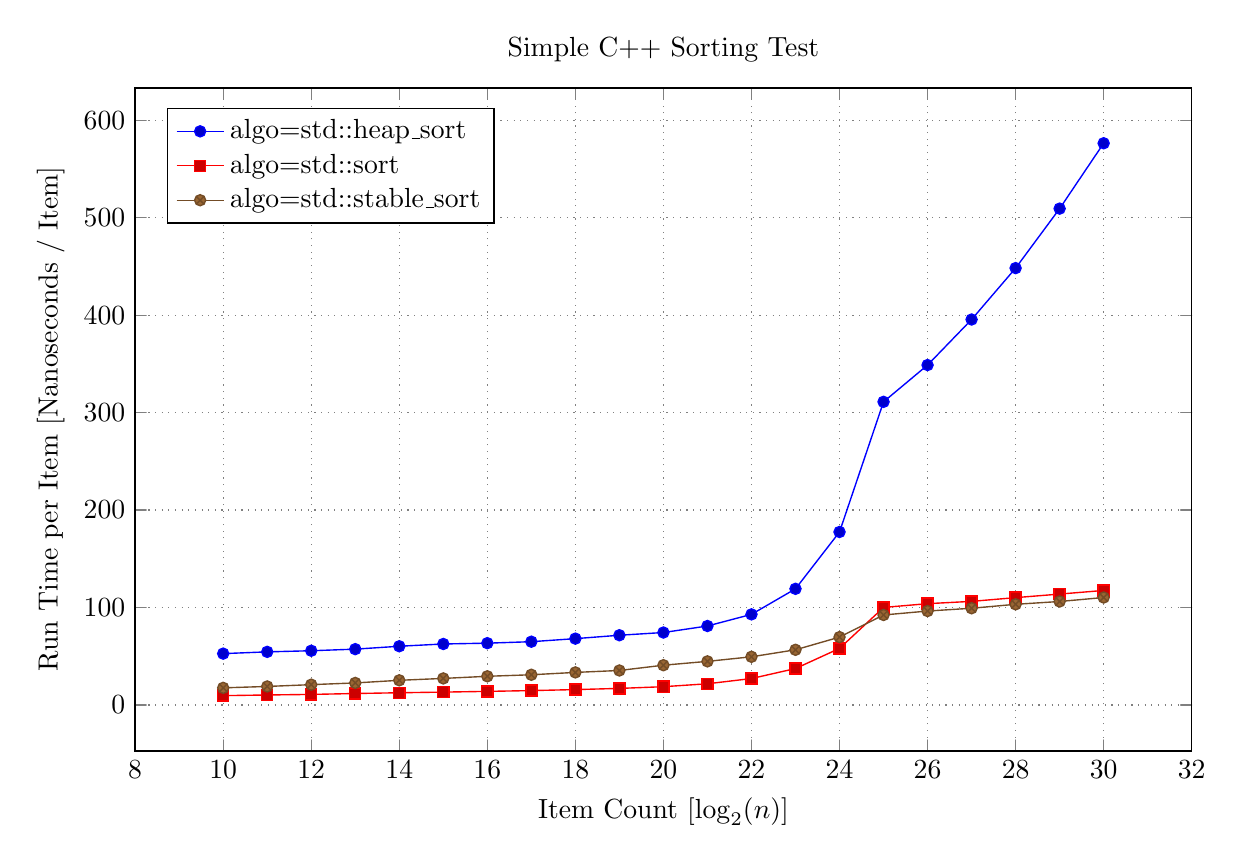
\begin{tikzpicture}
  \begin{axis}[
    title={Simple C++ Sorting Test},
    xlabel={Item Count [$\log_2(n)$]},
    ylabel={Run Time per Item [Nanoseconds / Item]},
    ]

    %% MULTIPLOT(algo) SELECT LOG(2, size) AS x, MEDIAN(time / repeats / size * 1e9) AS y, MULTIPLOT
    %% FROM stats GROUP BY MULTIPLOT,x ORDER BY MULTIPLOT,x
    \addplot coordinates { (10,52.6541) (11,54.4712) (12,55.6132) (13,57.2541) (14,60.2207) (15,62.5536) (16,63.3866) (17,64.8955) (18,68.0408) (19,71.5148) (20,74.3139) (21,80.9988) (22,92.9332) (23,119.146) (24,177.475) (25,310.999) (26,348.729) (27,395.465) (28,448.193) (29,509.227) (30,576.299) };
    \addlegendentry{algo=std::heap\_sort};
    \addplot coordinates { (10,9.53844) (11,10.2281) (12,10.8056) (13,11.73) (14,12.5076) (15,13.1773) (16,13.9202) (17,14.7259) (18,15.7581) (19,16.9725) (20,18.7205) (21,21.719) (22,27.0947) (23,37.3578) (24,58.0028) (25,100.04) (26,103.915) (27,106.265) (28,110.105) (29,113.754) (30,117.47) };
    \addlegendentry{algo=std::sort};
    \addplot coordinates { (10,17.5403) (11,18.9741) (12,20.8212) (13,22.5908) (14,25.2842) (15,27.2218) (16,29.3958) (17,30.9679) (18,33.3819) (19,35.364) (20,40.7699) (21,44.7148) (22,49.4075) (23,56.5833) (24,69.603) (25,92.3091) (26,96.3424) (27,99.2067) (28,103.255) (29,106.148) (30,110.22) };
    \addlegendentry{algo=std::stable\_sort};

  \end{axis}
\end{tikzpicture}
\end{center}

\begin{table}\centering
\begin{tabular}{l|rrr}
$n$ & \texttt{std::sort} & \texttt{std::stable\_sort} & STL heap sort \\ \hline
%% TABULAR REFORMAT(col 1-3=(precision=1) row 0-100=(min=bold))
%% SELECT '$2^{' || FLOOR(LOG(2, size)) || '}$' AS x,
%% (SELECT MEDIAN(time / repeats / size * 1e9) FROM stats s1 WHERE s1.algo='std::sort' AND s1.size = s.size GROUP BY s1.size),
%% (SELECT MEDIAN(time / repeats / size * 1e9) FROM stats s1 WHERE s1.algo='std::stable_sort' AND s1.size = s.size GROUP BY s1.size),
%% (SELECT MEDIAN(time / repeats / size * 1e9) FROM stats s1 WHERE s1.algo='std::heap_sort' AND s1.size = s.size GROUP BY s1.size)
%% FROM stats s
%% GROUP BY s.size ORDER BY s.size
$2^{10}$ &  \bf 9.5 &      17.5 &  52.7 \\
$2^{11}$ & \bf 10.2 &      19.0 &  54.5 \\
$2^{12}$ & \bf 10.8 &      20.8 &  55.6 \\
$2^{13}$ & \bf 11.7 &      22.6 &  57.3 \\
$2^{14}$ & \bf 12.5 &      25.3 &  60.2 \\
$2^{15}$ & \bf 13.2 &      27.2 &  62.6 \\
$2^{16}$ & \bf 13.9 &      29.4 &  63.4 \\
$2^{17}$ & \bf 14.7 &      31.0 &  64.9 \\
$2^{18}$ & \bf 15.8 &      33.4 &  68.0 \\
$2^{19}$ & \bf 17.0 &      35.4 &  71.5 \\
$2^{20}$ & \bf 18.7 &      40.8 &  74.3 \\
$2^{21}$ & \bf 21.7 &      44.7 &  81.0 \\
$2^{22}$ & \bf 27.1 &      49.4 &  92.9 \\
$2^{23}$ & \bf 37.4 &      56.6 & 119.1 \\
$2^{24}$ & \bf 58.0 &      69.6 & 177.5 \\
$2^{25}$ &    100.0 &  \bf 92.3 & 311.0 \\
$2^{26}$ &    103.9 &  \bf 96.3 & 348.7 \\
$2^{27}$ &    106.3 &  \bf 99.2 & 395.5 \\
$2^{28}$ &    110.1 & \bf 103.3 & 448.2 \\
$2^{29}$ &    113.8 & \bf 106.1 & 509.2 \\
$2^{30}$ &    117.5 & \bf 110.2 & 576.3 \\
% END TABULAR SELECT '$2^{' || FLOOR(LOG(2, size)) || '}$' AS x, (SELECT MEDI...
\end{tabular}
\caption{Runtime per element for different sorting implementation, median of 15 runs.}
\end{table}

\begin{comment}
% TEXTTABLE SELECT COUNT(*), SUM(time) FROM stats
+-------+--------------+
| count |          sum |
+-------+--------------+
|   945 | 24504.381188 |
+-------+--------------+
% END TEXTTABLE SELECT COUNT(*), SUM(time) FROM stats
\end{comment}

\end{document}

%%%%%%%%%%%%%%%%%%%%%%%%%%%%%%%%%%%%%%%%%%%%%%%%%%%%%%%%%%%%%%%%%%%%%%%%%%%%%%%%
